\subsubsection{Introduction}

The aim of part A is to implement the optimisation of the classification task
using the pretrained ResNet50 model. Fine-tuning based transfer learning is to
be utilised in order to apply the pretrained model to the required task, i.e.
classifying the Food-101 dataset.

\subsubsection{Rational}

Utilising a pretrained model can be useful as a fast way of deploying a neural
network. When using a small dataset, getting high test accuracy can be difficult
to achieve. Transfer learning can be utilised in order to improve the achieved
accuracy. By training only the output layers of the model on the new dataset,
the model can be trained to classify the new dataset to a high degree of
accuracy.

Another benefit of transfer learning is the training time. As the model is
pretrained, and only certain layers are required to be retrained on the new
dataset, the model can be trained in much fewer epochs, meaning that it will
train much quicker than an untrained or newly developed model.

\subsubsection{Design}

The Food-101 dataset is loaded from Google drive in the same way as Question 1.
Once loaded, the ``ImageDataGenerator'' for the training data must have the
``resnet50.preprocess\_input'' function applied. No preprocessing is to be done
to the validation or the test images. The ``flow\_from\_directory'' function is
again used to pull the images from google drive.

The base model for this problem is the keras ``ResNet50'' model. This model
takes the input arguments ``include\_top'', ``weights'', and ``input\_shape''.
Include top defines whether the classifier section of the model is included. As
this problem calls for transfer learning to be applied, this value is set to
False. The weights argument defines what data the model is trained on. Again,
the problem specifies that the ResNet50 model is trained on the ``imagenet''
weights. Finally, the input shape is the dimensions of the input data, which in
this case is 224x224x3.

\begin{figure}[H]
	\centering
	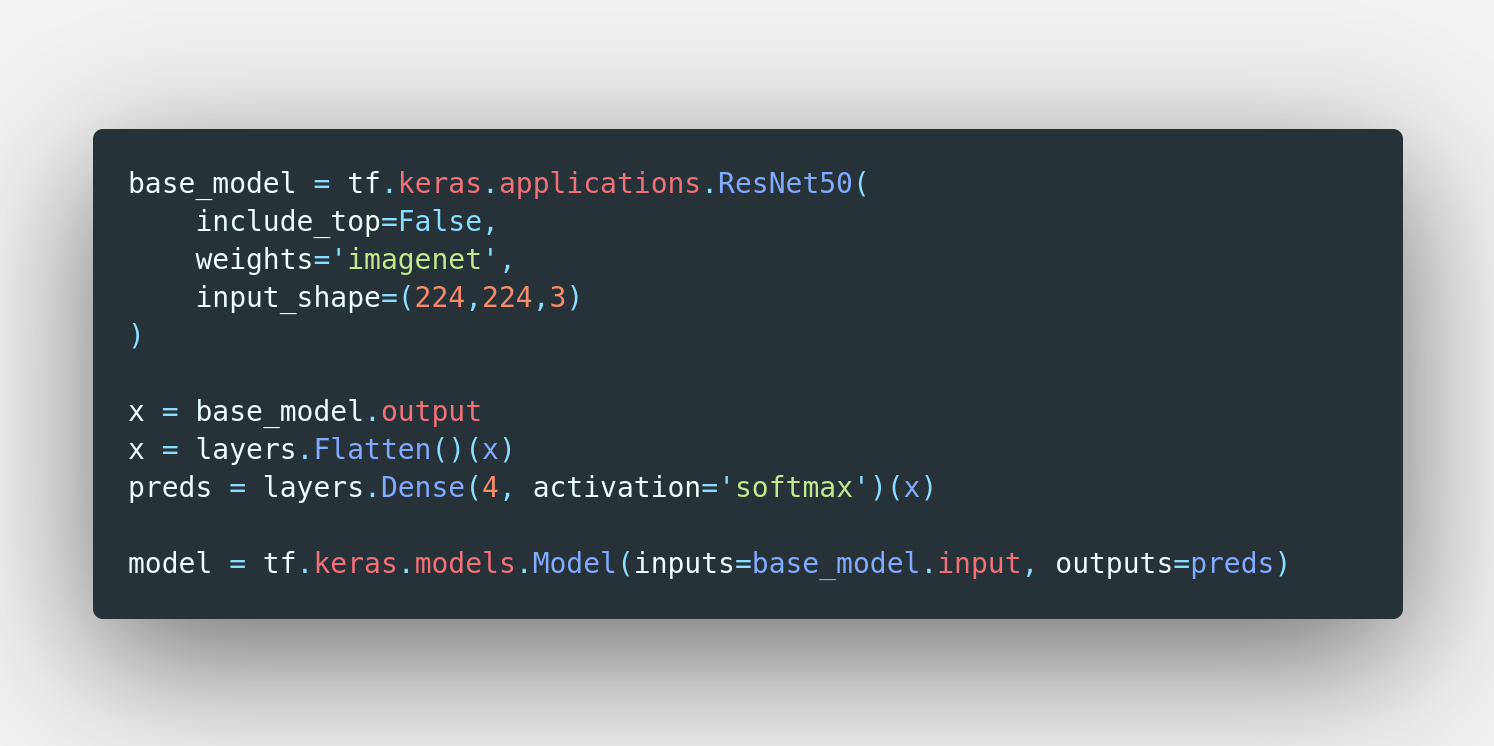
\includegraphics[width=0.8\textwidth]{images/Code/transfer}
	\caption{Transfer Learning Model}
	\label{fig:images-Code-transfer}
\end{figure}

Freezing was used in order to ensure that only the top ``res5c'' block, and the
added classifier block were trainable. This can be seen implemented in Figure
\ref{fig:freeze}.

\begin{figure}[H]
	\centering
	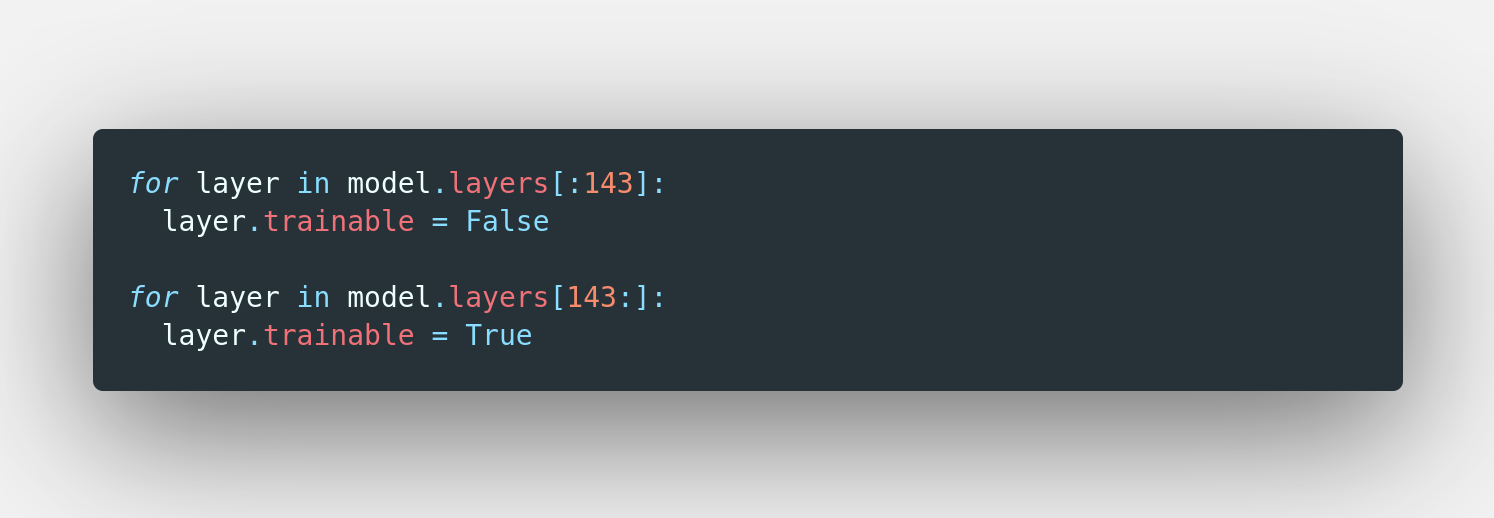
\includegraphics[width=0.8\textwidth]{images/Code/freeze}
	\caption{Freezing the Lower ResNet Layers}
	\label{fig:freeze}
\end{figure}

\subsubsection{Testing}

Testing of the transfer learning portion of this assignment involved only the
addition of the ``Flatten'' and ``Dense'' layers, and as such, no comparisons
between hyperparameters have been made.

\subsubsection{Results}

The final number of layers of the model can be seen in Figure \ref{fig:q2model}.
The added layers, i.e. the ``Flatten'' and ``Dense'' layers are the final output
layers, with the Dense layer classifying the images into one of four classes.

\begin{figure}[H]
	\centering
	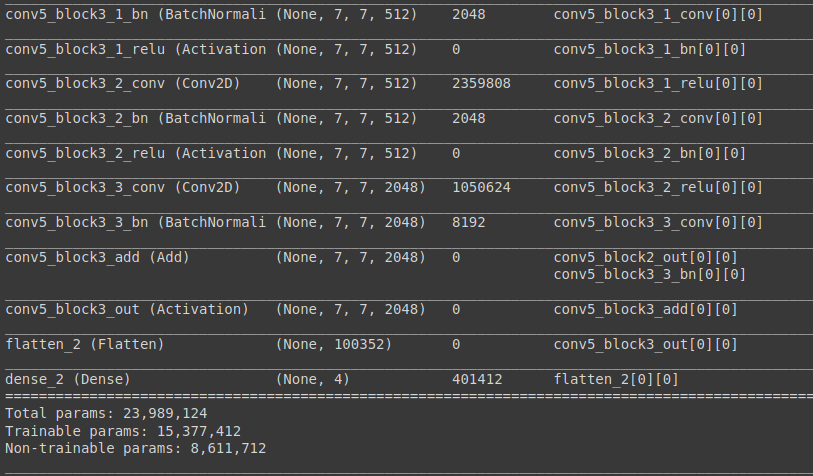
\includegraphics[width=0.8\textwidth]{images/q2/model}
	\caption{Model Summary (Final Layers)}
	\label{fig:q2model}
\end{figure}

There is an obvious difference between the training accuracy and the validation
accuracy, as shown in Figure \ref{fig:q2acc}, and it is clear from this graph
and from the final test results that the model is not overfitting.

\begin{figure}[H]
	\centering
	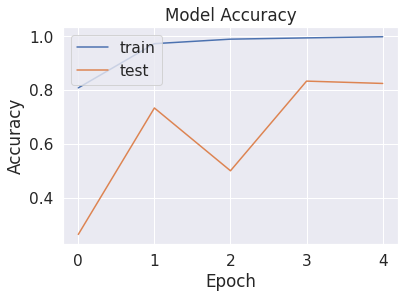
\includegraphics[width=0.8\textwidth]{images/q2/accuracy}
	\caption{Validation and Training Accuracy}
	\label{fig:q2acc}
\end{figure}

The loss for this model, as shown for both the training and validation sets in
Figure \ref{fig:q2loss}, is very low.
Over 5 epochs it can be seen how quickly the value decreases to almost zero.

\begin{figure}[H]
	\centering
	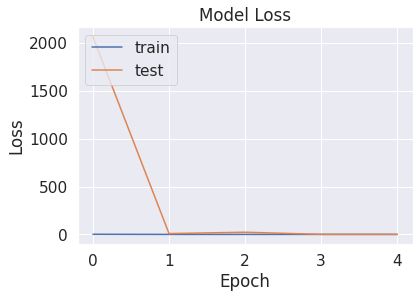
\includegraphics[width=0.8\textwidth]{images/q2/loss}
	\caption{Validation and Training Loss}
	\label{fig:q2loss}
\end{figure}

The final test results from the model can be seen in Figure
\ref{fig:q2results}. The precision has an average value of 83\%, while the
recall has an average value of 86\%. For such a short training time, this value
is much higher than that of Question 1. The highest precision value is for the
``Waffles'' class, however, the recall for this class is the lowest. The highest
recall value is for the ``Omlette'' class, but this has the lowest
precision value. The highest overall value by f1-score is for the ``Hamburger''
class, with a precision value of 91\%, and a recall value of 89\%.

\begin{figure}[H]
	\centering
	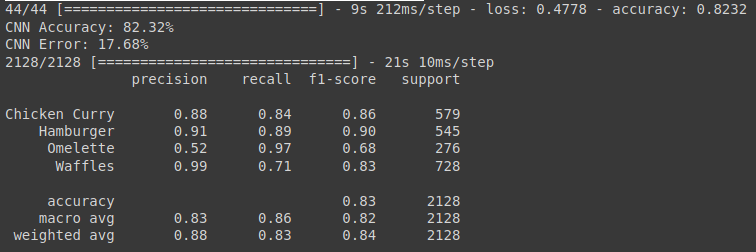
\includegraphics[width=0.8\textwidth]{images/q2/results}
	\caption{Model Testing Results}
	\label{fig:q2results}
\end{figure}

The confusion matrix shows the ``Waffles'' class, labeled as ``3'', as having
the
greatest number of correctly identified samples, while the ``Hamburger'' and
``Chicken Curry'' classes,
labelled ``1'' and ``0'' respectively, as having the least number of
incorrectly identified samples.

\begin{figure}[H]
	\centering
	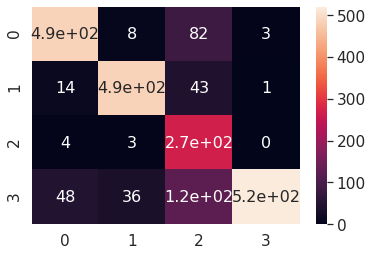
\includegraphics[width=0.8\textwidth]{images/q2/matrix}
	\caption{Confusion Matrix}
	\label{fig:q2matrix}
\end{figure}

The overall training time of this model was 154.2878 seconds. This would give a
value of 0.643lbs of CO2 equivalent emissions. This is much lower than the
developed baseline model in Question 1, and with a much higher output accuracy.
